\subsubsection{Sort}
The Sort controller lets users perform the Quicksort and Mergesort algorithms on arrays.
\begin{figure}[H]
    \centering
    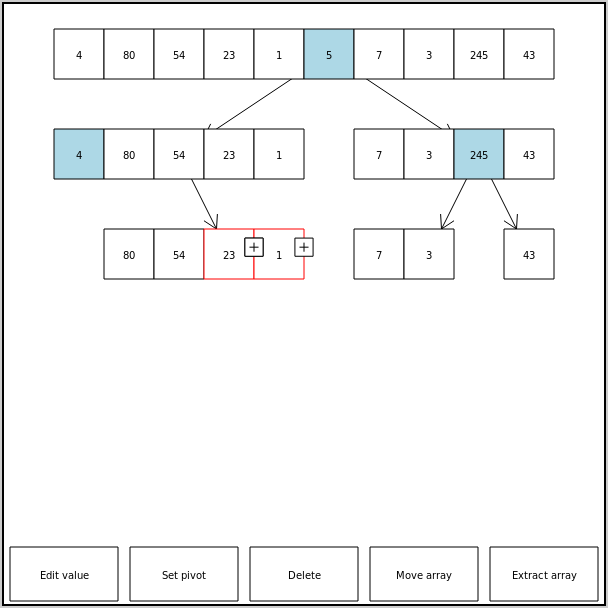
\includegraphics[width=0.7\linewidth]{/graphdrawer/sortui}
    \caption{Sort - user interface}
    \label{fig:graphdrawerSortUserInterface}
\end{figure}
The following properties can be determined by the optional configuration object:
\begin{enumerate}
    \item \code{sortType}, determines which algorithm to use. Can either be \code{"Mergesort"} or \code{"Quicksort"}. The default value is \code{"Quicksort"}.
    \item \code{bsf}, button-size-factor, determines how large the "+" buttons between nodes are. The default value is 3.
    \item \code{pivotColor}, determines which fill color nodes which are marked as a pivot have.
    \item \code{selectedColor}, determines which stroke color nodes which are selected will have.
    \item \code{extractType}, determines node position relative to other nodes when extracting nodes from an array. Possible values are \code{"vSorter"} which means the nodes are positioned based on their value, from low to high, and \code{"xSorter"} which positions them based on their x-position in the world.
    \item \code{joinType}, determines node position relative to other nodes when joining the nodes from different arrays to a new array. Possible values are \code{"vSorter"} and \code{"xSorter"}.
    \item \code{steps}, contains information about the starting array which the student needs to sort. It can also contain information about all of the actions one of the algorithms performed to sort the array.
\end{enumerate}
The \code{mouseDownHandler} function has four parts. It first checks if the world is empty. If it is, the first click creates the first node and array. If it is not empty, then it checks if any of the buttons were clicked. The buttons can only be clicked if they are visible, and they are made visible when the user selects one or more nodes. Only one node can be marked as \code{selected} (marked by + buttons \ref{fig:graphdrawerSortUserInterface}), but several can be in the selection list (marked by a red border \ref{fig:graphdrawerSortUserInterface}). When the user selects a node, the "Edit value", "Set pivot" and "Delete" buttons are shown. If the selection list contains nodes from only one array, the "Move array" and "Extract array" buttons are also shown. If the \code{sortType} is \code{"Mergesort"} and the selection list contains nodes from at least one array, then the "Join" button is also shown. If no button is clicked, and the user is trying to move an array, the array will be moved to the position of the interaction event. Finally, if nothing else happened, the selected node and the selection list is updated based on which nodes the user interacts with. When the user clicks and holds down their mouse button, the controller will start tracking which nodes are under the cursor. When the button is released, any node which was under the cursor will be in the selection list, and the last node from the list will be the selected node.
\\[11pt]
Arrays do not exist in the GraphDrawer's world. They are therefore only a part of the Sort controller. The controller has a reference to an array of array objects. The array objects contain a reference to every node in the array, the position of the array, and a list of other arrays which the array has a connection to. When an array is created, its position is set to the position of the first node. This is done so that the array will not move when more nodes are added to it. When a node is added to the array, all of the other nodes in the array will have an invalid position. To fix this, the node is first placed at the correct index, and then every node in the array is positioned according to their index in the reference array. When a node is removed, the same steps are performed. Because arrays do not exist in the GraphDrawer, edges between them also do not exist. Any link between two arrays is an edge between the nodes closest to the center of the arrays. This is achieved by updating the link when a node is added or removed from the array.
\\[11pt]
Even though all the controllers have a property with the name \code{steps}, the format does not have to be the same. Graph0 imports and exports the whole state of the graph after every operation. The steps in Sort contain information about which operation was performed, and on which elements. E.g. \code{{ type: "Split", list: [], left: [], right: [], ...}}. The sort controller can export and parse the following step types: "Initial", "Split", "Merge", "Complete". The initial step is used to describe the starting array. The split and merge steps are used to show what operation was performed, and its result. Because the exported steps also follow this format, it is possible that the student did something which is not considered a valid operation, e.g., split one array to four new arrays. To handle this, the complete step is used. If a student performs an invalid operation, the complete graph (similar to Graph0) is exported instead of an operation. The following is a list of all the required properties for every step type:
\begin{enumerate}
    \item \code{"Initial"}
    \begin{itemize}
        \item \code{list}, contains all the nodes in the array which should be sorted. The list should only contain the node values, because the node objects are created by the import function.
    \end{itemize}
    \item \code{"Split"}
    \begin{itemize}
        \item \code{list}, contains all the nodes in the array which should be split. The list should only contain node values.
        \item \code{left} and \code{right}, contains the nodes which are either placed in the left or the right array. At least one of them is required. One of them could be undefined, because splitting an array on a pivot, might only give one new array if a non-optimal pivot was picked.
        \item \code{pivot}, determines which node is the pivot node. If \code{sortType} is \code{"Mergesort"} this should be \code{undefined}. The student is able to mark more than one node as the pivot, however, if that happens, the operation is invalid, and the step type will be \code{"Complete"} instead.
    \end{itemize}
    \item \code{"Merge"}
    \begin{itemize}
        \item \code{merged}, contains the result of the merge operation. 
        \item \code{list1}, contains the node values from one of the lists which is being merged.
        \item \code{list2}, contains the node values from the other list which is being merged.
        \item \code{pivot}, if the \code{sortType} is \code{"Quicksort"} this is the node which is used as the pivot for the merge. 
    \end{itemize}
    \item \code{"Complete"}
    \begin{itemize}
        \item \code{arrays}, should be an array containing all of the arrays. This does not enforce any restrictions on the arrays, e.g., one array can link to more than two other arrays.
    \end{itemize}
\end{enumerate}